\documentclass[mathserif, 10pt]{beamer}
\usepackage[utf8]{inputenc}
\usepackage{amsmath, amsfonts}
\usepackage{appendixnumberbeamer}


\title[A Glance into Flavour Physics...]{A Glance into Flavour Physics \\with Effective Field Theories\\ and Machine Learning}
\author[Jorge Alda]{Jorge Alda,\\ Universidad de Zaragoza/CAPA\\
Università degli Studi di Padova/INFN \hspace{2em} \texttt{jalda@unizar.es} }

\date[PhD Thesis]{28th April 2022}



\usetheme{Zaragoza}
\usecolortheme{Unizar}
\titlepagelogoA{
\includegraphics[width=6cm]{logos/CAPA.png}}
\titlepagelogoB{
\includegraphics[width=4cm]{logos/dftuz2.png}}


\newcommand\colorcite[1]{{\scriptsize\color{blue}#1}}

\begin{document}
\begin{frame}[noframenumbering,plain]

\titlepage

\end{frame}

\begin{frame}
    \frametitle{Publication List}

    \begin{itemize}
        \item J. Alda, J. Guasch, S. Peñaranda,
              \textit{Some Results on Lepton Flavour Universality Violations,}\\
              Eur. Phys. J. C 79.7 (2019), p.588, arXiv:1805.03636 [hep-ph].
        \item J. Alda, J. Guasch, S. Peñaranda, \textit{Anomalies in B meson decays: A phenomenological approach,}\\
              Eur. Phys. J. Plus 137 (2022), p.217, arXiv: 2012.14799 [hep-ph].
        \item J. Alda, J. Guasch, S. Peñaranda,
              \textit{Using Machine Learning techniques in phenomenological studies in flavour physics,}\\
              arXiv:2109.07405 [hep-ph].
        \item J. Alda, A. W. M. Guerrera, S. Peñaranda, S. Rigolin,
              \textit{Leptonic Meson Decays into invisible ALP,}\\
              arXiv:2111.02536 [hep-ph].
    \end{itemize}

\end{frame}

\begin{frame}
    \frametitle{Part I: $B$ physics}
\end{frame}

\begin{frame}
    \frametitle{$B$ anomalies}

    Flavour-changing neutral currents $b \to s \ell^+ \ell^-$, with $\ell = e, \mu$.
    \begin{itemize}
        \item Universality ratios $R_{K^{(*)}}$
              $$R_{K^{(*)}} = \frac{\mathrm{BR}(B\to K^{(*)}\mu^+ \mu^-)}{\mathrm{BR}(B\to K^{(*)}e^+ e^-)}\,, $$
              In the SM, theoretically clean, and $R_{K^{(*)}}=1$.\\
              LHCb measurements\footnote{R. Aaij \textit{et al.} (LHCb) arXiv:2103.11769, arXiv:1705.05802}:
              \begin{itemize}
                  \item $R_{K^+} = 0.846^{+0.042}_{-0.039}{}^{+0.013}_{-0.012}$,
                  \item $R_{K^{*0}} = 0.685^{+0.113}_{-0.069}\pm0.047$. ($3.1\,\sigma$ tension)
              \end{itemize}
        \item Angular observables for $B\to K^* \ell^+\ell^-$: $P'_4$, $P'_5\ldots$
        \item Also $B_s \to \phi \mu^+ \mu^-$ decays.
    \end{itemize}

\end{frame}

\begin{frame}
    \frametitle{$B$ anomalies}
    Flavour-changing charged currents $b\to c \ell \nu$, with $\ell = e/\mu, \tau$.
    \begin{columns}
        \begin{column}{0.55\textwidth}

            \begin{itemize}
                \item Universality ratios $R_{D^{(*)}}$
                      $$R_{D^{(*)}} = \frac{\mathrm{BR}(B\to D^{(*)}\tau \nu)}{\mathrm{BR}(B\to D^{(*)}\ell \nu)}\,, $$
                      $$R_D = 0.340 \pm 0.027 \pm 0.013\,,$$
                      $$R_{D^*} = 0.295 \pm 0.011 \pm 0.008\,.$$
                      Combined tension of $3.08\,\sigma$.\footnotemark[1]
                \item Longitudinal polarization of $D^*$.
                \item Also $B_c \to J/\psi \ell\nu$ decays.
            \end{itemize}

        \end{column}
        \begin{column}{0.5\textwidth}
            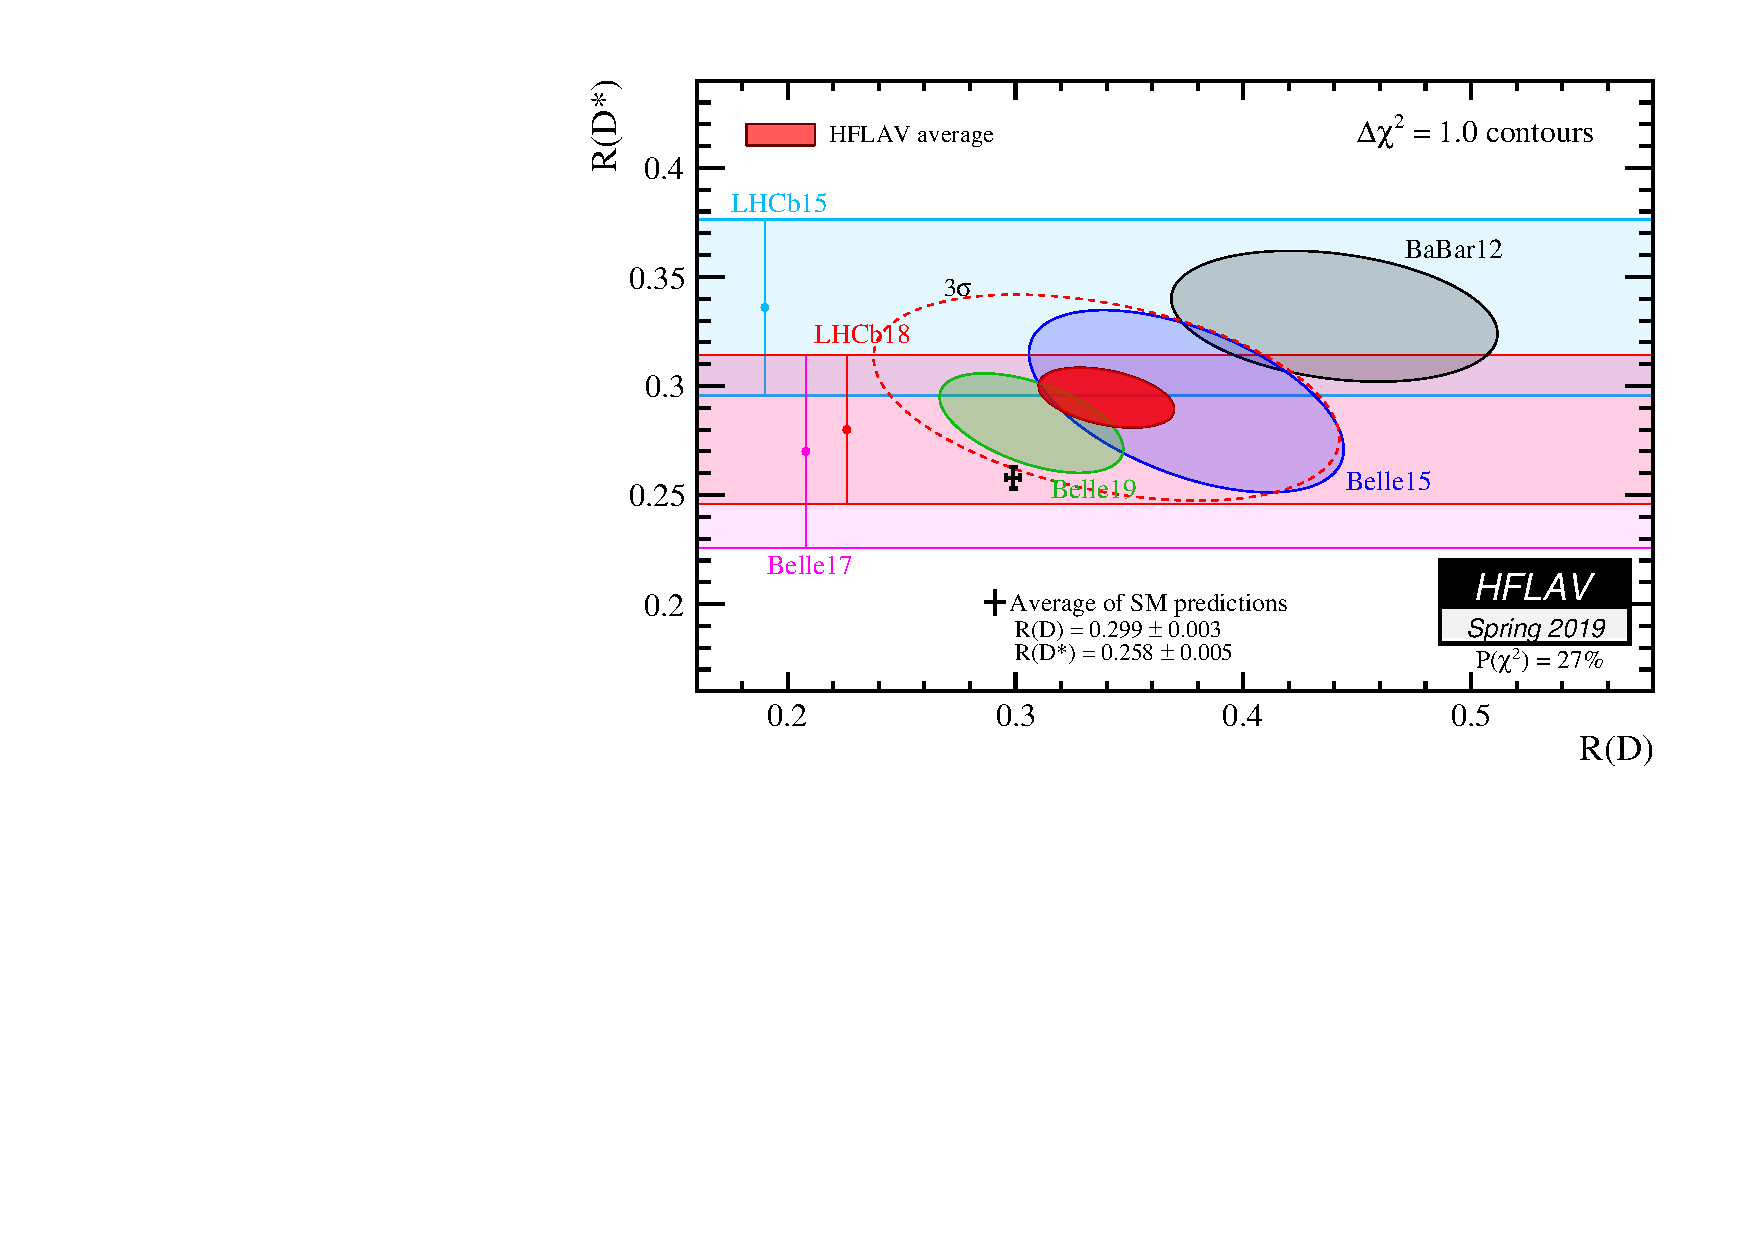
\includegraphics[width=\columnwidth]{figures/rdrds_spring2019.pdf}
        \end{column}
    \end{columns}
    \footnotetext[1]{Y. S. Ahmis \textit{et al.} (HFLAV) arXiv:1909.12524}
\end{frame}

\begin{frame}
    \frametitle{Effective Field Theories}

    Deviations from the SM predictions can be described in a systematic way using Effective Field Theories.



\end{frame}

\end{document}